\documentclass[../main.tex]{subfiles}

\begin{appendices}

\chapter{Acknowledgments}
\section{Concept, clock model, filter values and graphs}
Harald Hauglin, Chief engineer time & frequency metrology at Justervesenet was responsible for the following:
\begin{itemize}
	\item Describing the Clock model algorithm.
	\item The concept of CSAC SMACC (Chip scale atomic clock smart miniature atomic clock controller) that this work is built on.
	\item Created the graphs used in section \ref{gpsdata_test1}, \ref{test1_measurements}, \ref{gpsdata_test2}, \ref{test2_meaurements} and \ref{unplanned_disturb}.
	\item Filter reference values, both for clock model based filters and GPS based filters.
\end{itemize}

Mr. Matt Davis is the author of \texttt{jdutil.py}\cite{MATT_DAVIS}, a library written for converting dates and time to MJD and back. Permission to use the jdutil.py was granted by Mr. Davis. The correspondence with Mr. Davis is included in the appendix under \ref{davis_email}.


\chapter{Clock model}\label{clock_model_harald}
Clock modelling and clock filters in the spoof proof clock controller
V 2.0 20161027 HHA

\section{Introduction}
The goal of clock modelling is to provide an estimate of two key parameters of the clock "state", the frequency offset and the clock drift, i.e. the rate of change of the frequency offset. The clock model will be used for two purposes: (1) As a reference for the clock frequency correction filter, in order to determine whether the current clock correction, as calculated and applied by the CSAC disciplining algorithm, is consistent with normal behavior of the clock; (2) In the case that a valid external disciplining pulse is lost, the model will be used to calculate the frequency corrections to be applied to the CSAC by the "spoof" proof clock controller. The model described below is a simple way of modelling the clock state, motivated by being easy to implement, more than being optimal for the task.  

\section{Input data for the clock model}
Input data for the clock model comes from the CSAC telemetry string, sampled nominally every second. The key data is contained in the field identified by "Steer". This is the CSAC disciplining algorithm's current estimate of the frequency correction (in relative units) that has to be applied to the CSAC microwave synthesizer to correct for the frequency error of the CSAC "physics package". Ref \cite{CSAC_USERGUIDE}. Sample telemetry string and explanation of the data fields below are from the CSAC User Guide[ref]. Note that the "Steer" value reported by the CSAC in disciplining mode is the frequency correction that is applied to make the CSAC in sync with the external applied reference pulse. If the reference pulse  is accurate – such as the 1 PPS pulse output from a properly operating GPS timing chip - then the negative "Steer" value is an estimate of the free-running CSAC  frequency offset, i.e. a calibration of the CSAC. 

As long as there is a valid and accurate reference pulse, a series of "Steer" values provide the basis for estimating the frequency offset of the CSAC, as well as its rate of change (drift). 

One should note that the PPS output from the GPS chip has substantial noise in the short term. In contrast, the CSAC itself is more stable than the GPS reference over timespans up to 10000 s \cite{CSAC_USERGUIDE}.  As a consequence, the steering corrections calculated by the CSAC are also noisy and that noise primarily due to noise in the reference pulse.  In order to provide good estimates of the clock state, it is useful to filter sampled steering data to remove the influence of noise. This will be described next. Figure \ref{telemetry_string_a} show an example telemetry string.

\begin{lstlisting}[caption={Example of a telemetry string received from the atomic clock},label={telemetry_string_a}]
0,0x0000,1209CS00909,0x0010,4381,0.86,1.573,17.62,0.996,28.26,-24,---,-1,1,1268126502,586969,1.0
\end{lstlisting} 

\begin{figure}[!htb]
  \centering
  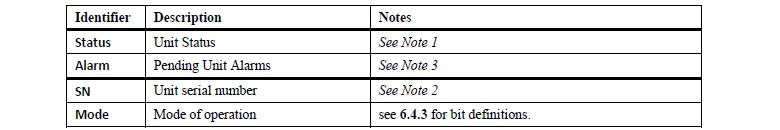
\includegraphics[width=1\textwidth]{csa_model_table6.png}
  \caption{Part 1 of table showing telemetry parameters. The table is taken from the SA.45's manual \cite{CSAC_USERGUIDE}}
  \label{phase_offset}
\end{figure} 

\begin{figure}[!htb]
  \centering
  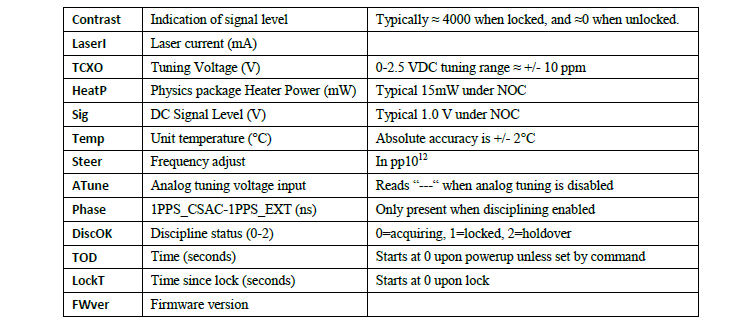
\includegraphics[width=1\textwidth]{csa_model_table6-2.png}
  \caption{Part 2 of table showing telemetry parameters. The table is taken from the SA.45's manual \cite{CSAC_USERGUIDE}}
  \label{phase_offset}
\end{figure}  

\newpage 
\section{Smoothing of sampled frequency steering data and estimates of the clock state}
The frequency steer filter will be based on smoothed values of current and previous "steer" data from the CSAC telemetry string.
The method described here is a very simple approach, primarily chosen for its ease of implementation. It is based on the assumption that "Steer" values are sampled at regular intervals. The design of an optimized approach for clock parameter estimation is way beyond the scope of this work. Calculation of smoothed values. Smoothed values of the clock steering correction are calculated using an exponential filter. Input to the calculation is the current sampled "Steer" value, steer\_current,  along with its associated timestamp (in mjd), t\_current. The exponential filter has a parameter, w, whose inverse is the weight that each new sampled value adds to the existing smooth value:

\begin{displaymath}
	steer\_smooth\_current = \frac{w-1}{w} steer\_smooth\_previous + \frac{1}{w} steer\_current
\end{displaymath}

Smoothing is initialized by setting steer\_smooth\_previous = steer\_current .
Since the current smoothed value of the steering parameter is a weighted average of all previous samples as well, it effectively "lags" behind in time. The effect of this lag can be calculated by applying the same exponential smoothing to the associated timestamps 

\begin{displaymath}
	t\_smooth\_current = \frac{w-1}{w} t\_smooth\_previous + \frac{1}{w} t\_current  
\end{displaymath}

Again, smoothing is initialized by setting t\_smooth\_previous  = t>\_current. Updated smoothed values t\_smooth and steer\_smooth will be computed every time the telemetry string is read (about once per second). Representative data for sampled and smoothed "steer" values are shown in fig XXX. Daily updated clock model Smoothed values will be used to estimate the frequency drift. A simple approach that "works" is to use values at the start of every day and compare to the values from the previous day. Again, this is not an optimized approach. At the start of every new day set the following:

\begin{displaymath}
	t\_smooth\_today = t\_smooth\_current
	steer\_smooth\_today  = steer\_smooth\_current
\end{displaymath}

and label previous day's values t\_smooth\_yesterday and steer\_smooth\_yesterday. The drift of the steering parameter can be estimated as:

\begin{displaymath} 
   steer\_drift  = \frac{(steer\_smooth\_today – steer_smooth\_yesterday)}{(t\_smooth\_today – t\_smooth\_yesterday)}
\end{displaymath}

The predicted steering parameter for a given point in time t can now be computed as a simple linear relationship

\begin{displaymath}
	steer\_predicted (t) = steer\_smooth\_today + (t – t\_smooth\_today) * steer\_drift
\end{displaymath}

The output of this model is the predicted CSAC steering correction for a given point in time t. 

\section{Phase offset filter – fast timing filter}
The "fast" timing filter will check the value of the "Phase" CSAC telemetry phase field. The CSAC disciplining algorithm steers the clock so that the generated PPS output is in sync with the reference PPS input. The reference value for the phase offset filter is therefore 0. Limits for acceptable deviations from the reference value has to be based on normal noise in the phase data. A representative series of phase data is shown in figure \ref{phase_offset}. 
\begin{figure}
  \centering
  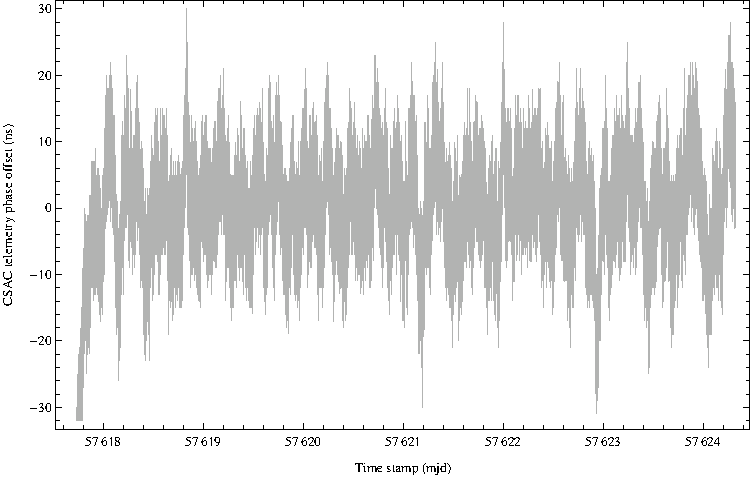
\includegraphics[width=1\textwidth]{clock_model_phase_offset.pdf}
  \caption{Figure shows phase offset in nanoseconds as measured by the CSAC}
  \label{phase_offset}
\end{figure} 
The filter parameter is a constant phase\_limit will be read from a configuration file. Flag for invalid timing will be raised when:

\begin{displaymath}
	abs(phase\_current) > phase\_limit
\end{displaymath}

Tentatively phase\_limit is set to 50 ns. 

\section{Frequency correction filter}
The frequency correction filter will check the value of the CSAC telemetry "steer" field and compare it to the steering correction predicted by the clock model. Limits for acceptable deviations from the predicted value has to be based on normal noise in the frequency steering data. A representative series of sampled steering data along with model predictions is shown in figure [xxxx].
Filtering of the current frequency steering can now be implemented as follows:

\begin{displaymath}
	Abs(steer\_current – steer\_predicted(t\_current)) > steer\_limit
\end{displaymath}

The parameter steer\_limit will be read from a configuration file. The limit is tentatively set to 50 based on the data below. Note that this is a relative frequency correction in units of ($10^{12}$), corresponding to rate of change of 0.05 ns/s in the timing output of the clock. 
\begin{figure}
  \centering
  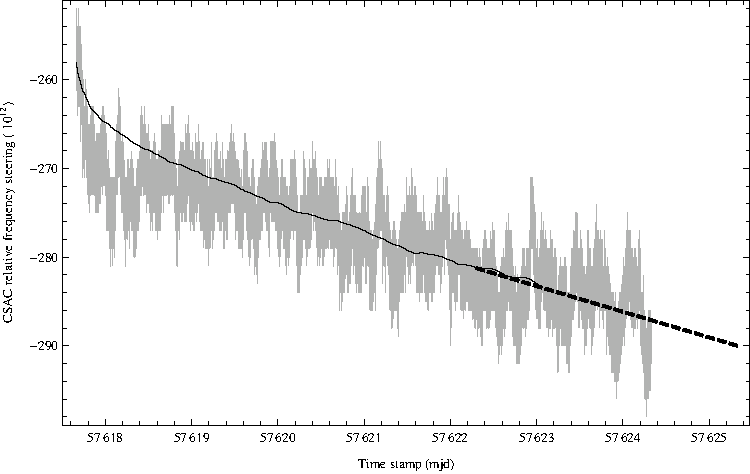
\includegraphics[width=1\textwidth]{csac_modelling_prediction.pdf}
  \caption{Sampled clock steering corrections (gray), smoothed values (black solid line) and predicted clock steering values (dashed). Sampled data at 1 s intervals have been smoothed using an exponential filter with filter parameter w = 100000.}
  \label{phase_offset}
\end{figure} 

\chapter{Data acquisition}
\section{CSAC Logger source code}\label{CL}
	\pythoncode{./source_files/csac_logger.py}
\section{GPS Logger source code}\label{GL}
	\pythoncode{./source_files/gps_logger.py}
\section{GPS Logger source code}\label{server_script}
	\pythoncode{./source_files/script_example.py}
	
\chapter{Sensor server software}
\section{Client}
\subsection*{sensor\_client.c}\label{sensor_client.c}
	\ccode{../server/sensor_client.c}
\subsection*{sensor\_client.h}\label{sensor_client.h}
	\ccode{../server/sensor_client.h}
\subsection*{client\_config.ini}
	\ccode{../server/client_config.ini}
\subsection*{query\_csac.py}
	\pythoncode{../server/query_csac.py}

\section{Server}
\subsection*{sensor\_server.c}
	\ccode{../server/sensor_server.c}\label{sensor_server.c}
\subsection*{sensor\_server.h}
	\ccode{../server/sensor_server.h}\label{sensor_server.h}
\subsection*{config.ini}
	\ccode{../server/config.ini}

\subsection*{sensor\_server\_common.h}
	\ccode{../server/sensor_server_common.h}\label{sensor_server_common.h}

\subsection*{session.c}
	\ccode{../server/session.c}\label{session.c}
\subsection*{session.h}
	\ccode{../server/session.h}

\subsection*{actions.c}
	\ccode{../server/actions.c}
\subsection*{actions.h}
	\ccode{../server/actions.h}

\subsection*{utils.c}
	\ccode{../server/utils.c}
\subsection*{utils.h}
	\ccode{../server/utils.h}

\subsection*{net.c}
	\ccode{../server/net.c}
\subsection*{net.h}
	\ccode{../server/net.h}

\subsection*{csac\_filter.c}
	\ccode{../server/csac_filter.c}
\subsection*{csac\_filter.h}
	\ccode{../server/csac_filter.h}
\subsection*{cfilter\_config.ini}
	\ccode{../server/cfilter_config.ini}
\subsection*{get\_telemetry.py}
	\pythoncode{../server/get_telemetry.py}

\subsection*{filters.c}
	\ccode{../server/filters.c}
\subsection*{filters.h}
	\ccode{../server/filters.h}

\subsection*{net.c}
	\ccode{../server/net.c}
\subsection*{net.h}\label{net.h}
	\ccode{../server/net.h}

\subsection*{gps\_serial.c}
	\ccode{../server/gps_serial.c}
\subsection*{serial.h}
	\ccode{../server/serial.h}

\subsection*{colors.h}
	\ccode{../server/colors.h}

\subsection*{config.h}
	\ccode{../server/config.h}

\subsection*{nmea.h}\label{nmea.h}
	\ccode{../server/nmea.h}

\subsection*{list.h}\label{list}
	\ccode{../server/list.h}

\subsection*{protocol.h}
	\ccode{../server/protocol.h}

\subsection*{makefile}
	\makecode{../server/makefile}

\chapter{Scripts}
	\section*{CSAC query source code}\label{query_csac}
		\pythoncode{../server/query_csac.py}
	\section*{MJD calculator}\label{get_mjd}
		\pythoncode{../server/get_mjd.py}	
	\section*{Script example}\label{script_example}
		\pythoncode{source_files/script_example.py}	

\section{Logger setup schematic}\label{CLS}
	 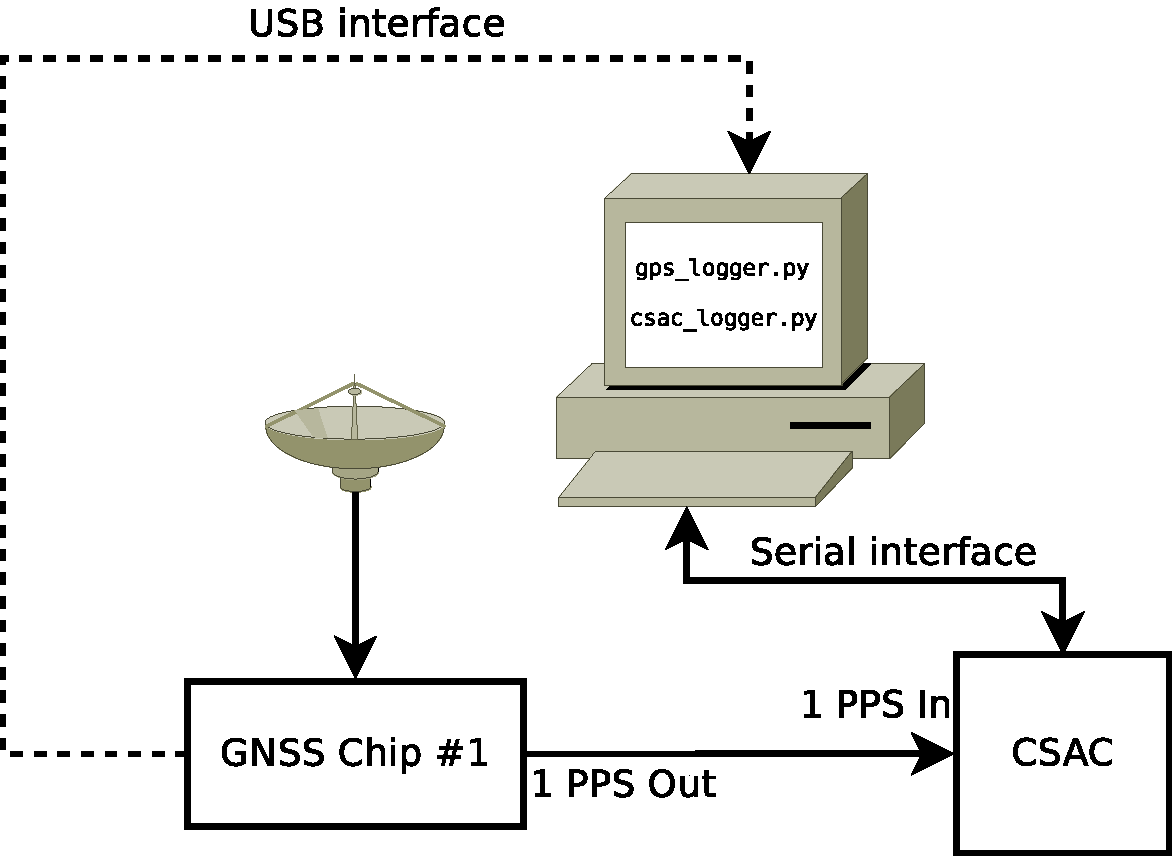
\includegraphics[scale=0.5]{csac_logger.pdf}

\chapter{E-mails}
\section{Correspondence with Mr. Davis}\label{davis_email}
\begin{Verbatim}[fontsize=\footnotesize ]

Hi Aril,

This would be fine, but you may want to take a look at the Astropy library
and see if their time package would meet your needs. It's certain to be
more robust and well tested. But if you'd like to use my module, please do.
http://docs.astropy.org/en/stable/time/index.html

Best,
Matt Davis

On Sun, Oct 23, 2016 at 2:25 PM Aril Schultzen <aschultzen@gmail.com> wrote:

> Hi!
>
> I am currently writing my master thesis in compsci and I wanted to ask you
> if it was OK if I used your library for converting dates to/from JD and MJD
>   (https://gist.github.com/jiffyclub/1294443) in my implementation? It
> will be used to convert time to MJD for a model and also for stamping logs.
> Your work will of course be acknowledge as your own.
>
> Kind regards
>
> Aril Schultzen
>
\end{Verbatim}

\chapter{Figures}
	\begin{figure}
	\centering
	  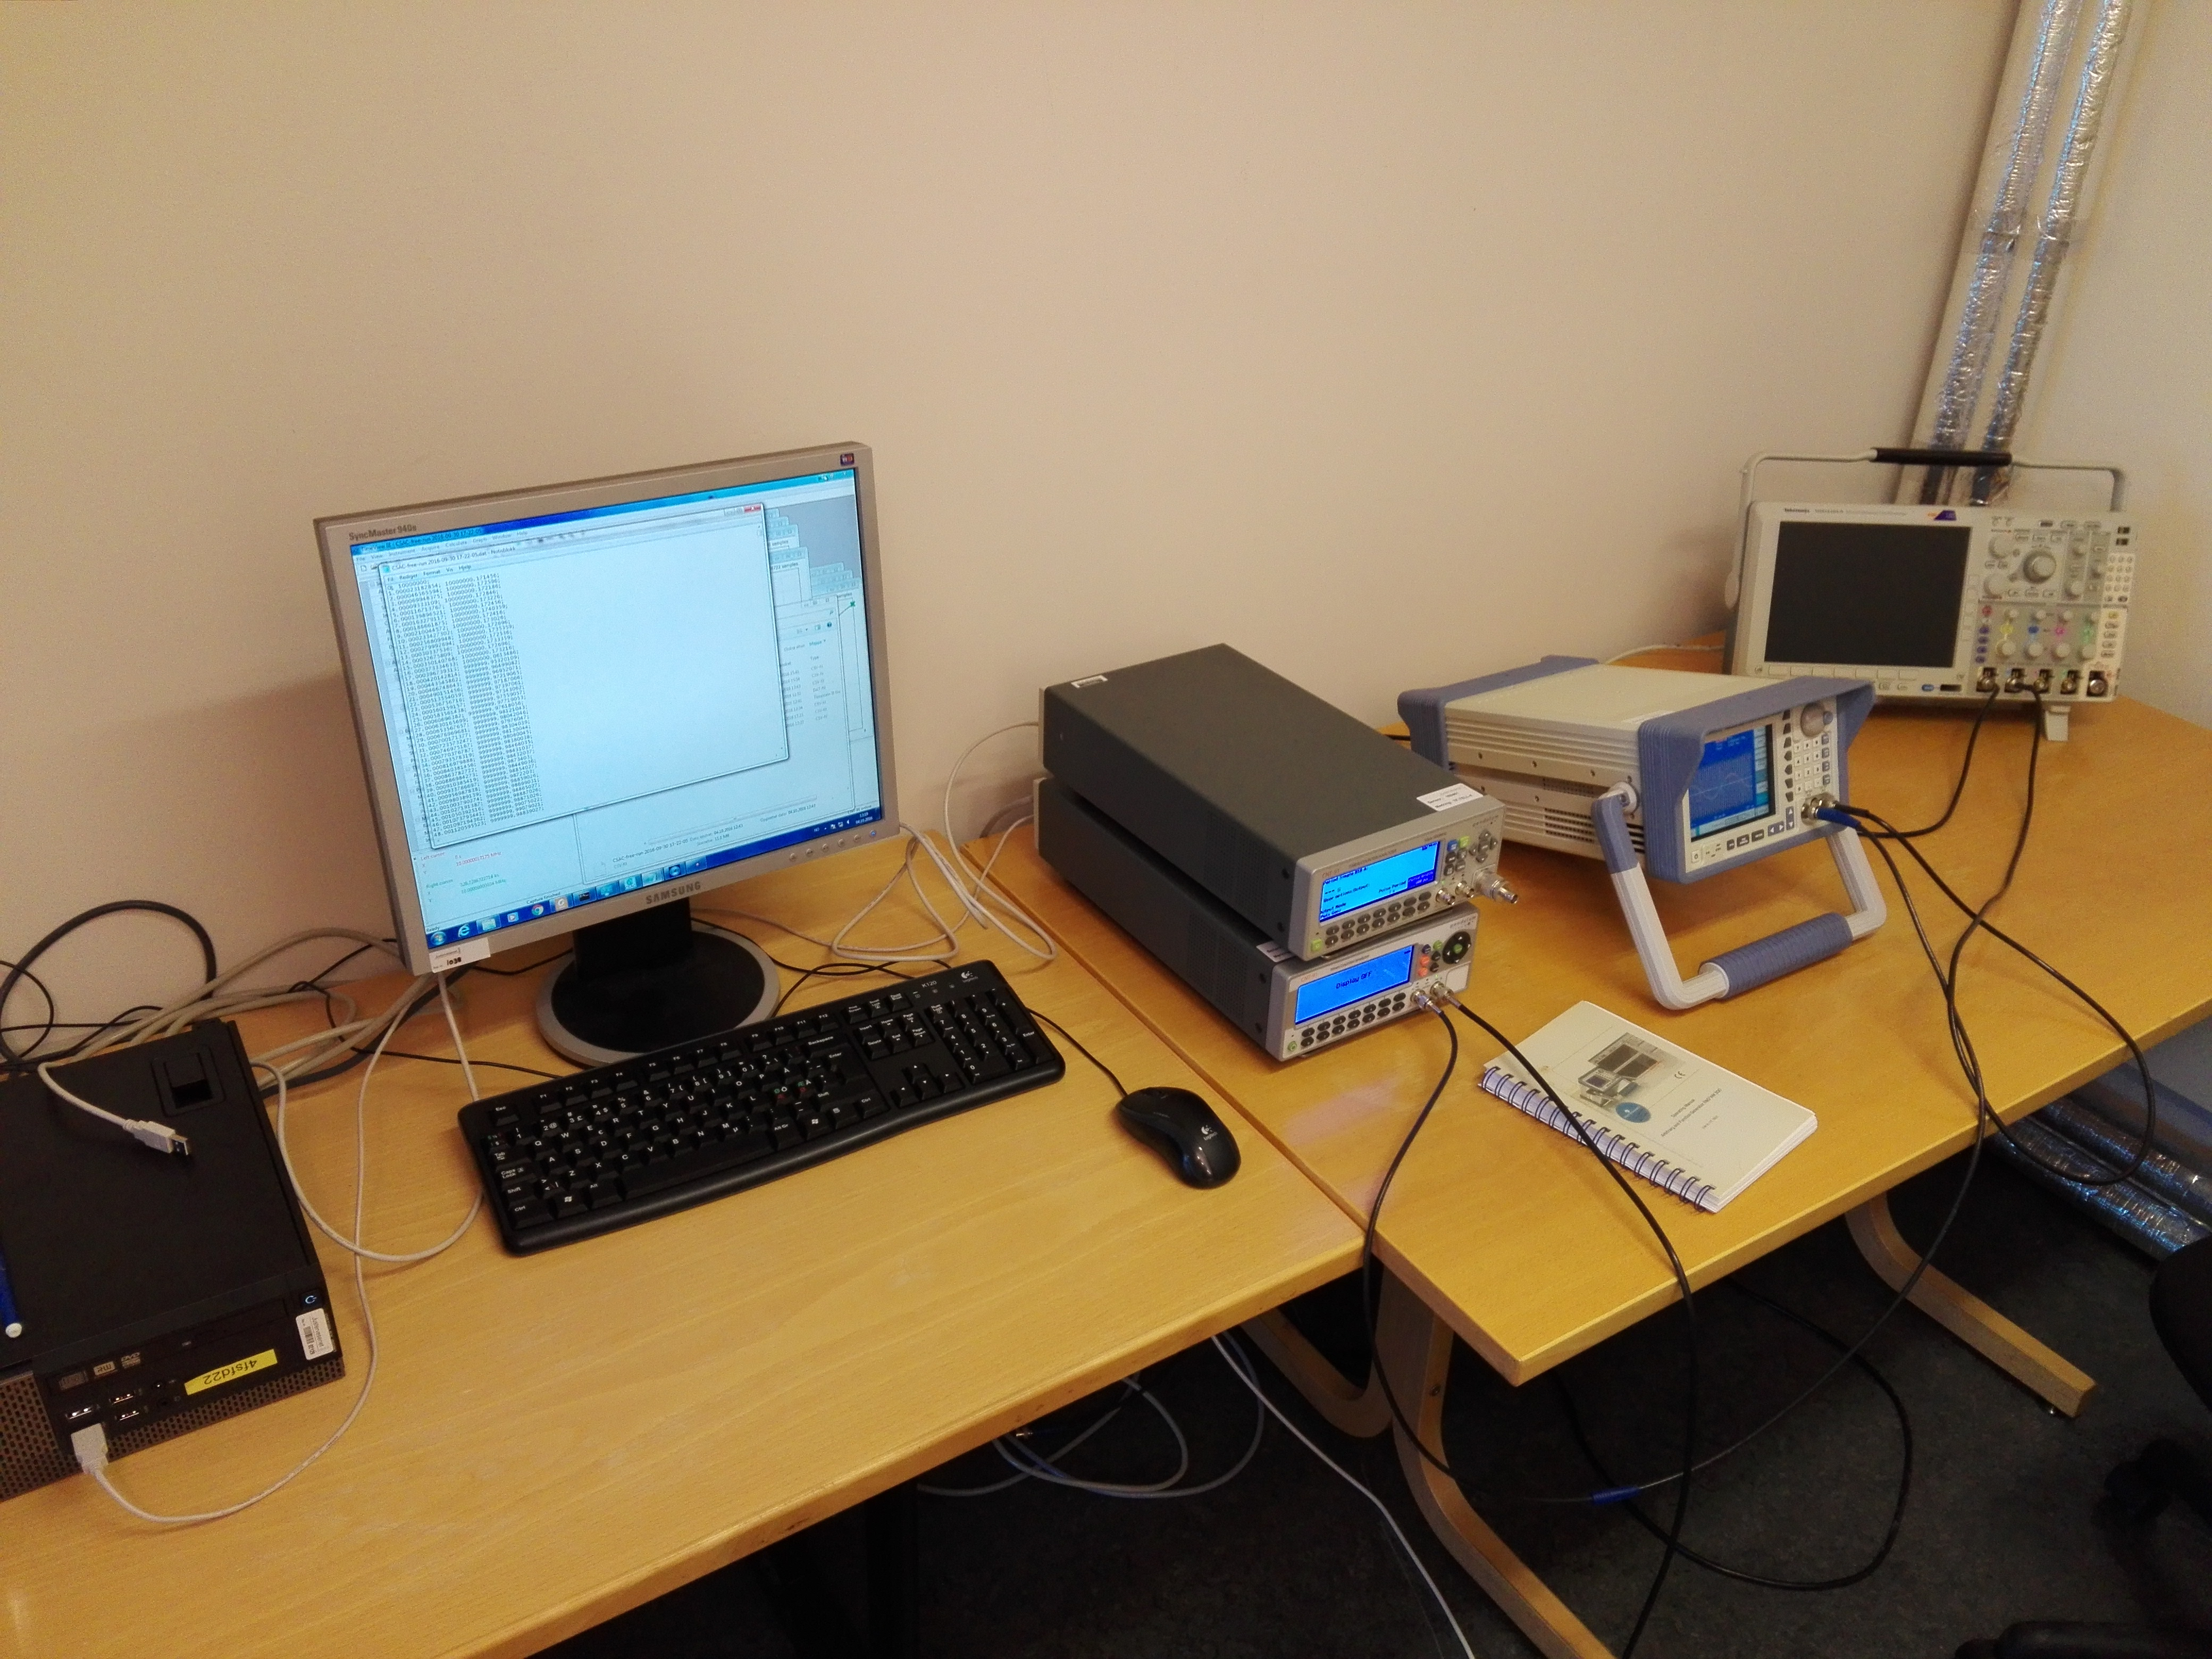
\includegraphics[scale=0.09]{lab_setup.jpg}
	   \caption[Photograph of the measuring setup]{Photograph of the system used to measure the 10 MHz output from the atomic clock. Not in the picture is the source of the 10 MHz reference.}
	   \label{lab_setup_photo}
	\end{figure}

\end{appendices}